\documentclass[
	% -- opções da classe memoir --
	12pt,				% tamanho da fonte
	openany,			% capítulos começam em pág ímpar (insere página vazia caso preciso)
  oneside,      % para impressão em página única. Oposto ao twoside (Nunca habilitar os dois!)
	%twoside,			% para impressão em recto e verso. Oposto a oneside (Nunca habilitar os dois!)
	a4paper,			% tamanho do papel. 
	% -- opções da classe abntex2 --
	%chapter=TITLE,		% títulos de capítulos convertidos em letras maiúsculas
	%section=TITLE,		% títulos de seções convertidos em letras maiúsculas
	%subsection=TITLE,	% títulos de subseções convertidos em letras maiúsculas
	%subsubsection=TITLE,% títulos de subsubseções convertidos em letras maiúsculas
	% -- opções do pacote babel --
	english,			% idioma adicional para hifenização
	french,				% idioma adicional para hifenização
	spanish,			% idioma adicional para hifenização
	brazil				% o último idioma é o principal do documento
	]{abntex2}

% ---
% Pacotes básicos 
% ---
\usepackage{lmodern}			  % Usa a fonte Latin Modern			
\usepackage[T1]{fontenc}		% Selecao de codigos de fonte.
\usepackage[utf8]{inputenc} % Codificacao do documento (conversão automática dos acentos)
\usepackage{lastpage}			  % Usado pela Ficha catalográfica
\usepackage{indentfirst}    % Indenta o primeiro parágrafo de cada seção.
\usepackage{color}				  % Controle das cores
\usepackage{graphicx}			  % Inclusão de gráficos
\usepackage{subfig}         % Sub-figuras
\usepackage{microtype}      % para melhorias de justificação
\usepackage{textcomp}       % Adiciona símbolo de trademark e outros ao T1
\usepackage{array}          % Usado nas tabelas com \newline
\usepackage{multirow}       % Define tabelas multirow
\usepackage{minted}
\usepackage{listings}       % Program listings
		
% ---
% Pacotes adicionais, usados apenas no âmbito do Modelo Canônico do abnteX2
% ---
\usepackage{lipsum}				% para geração de dummy text
% ---

% ---
% Pacotes de citações
% ---
\usepackage[brazilian,hyperpageref]{backref}	 % Paginas com as citações na bibl
\usepackage[alf]{abntex2cite}	% Citações padrão ABNT

% Copiado das configurações do LyX

%%%%%%%%%%%%%%%%%%%%%%%%%%%%%% LyX specific LaTeX commands.
%% Because html converters don't know tabularnewline
\providecommand{\tabularnewline}{\\}

%%%%%%%%%%%%%%%%%%%%%%%%%%%%%% User specified LaTeX commands.

% --- 
% CONFIGURAÇÕES DE PACOTES
% --- 

% ---
% Configurações do pacote backref
% Usado sem a opção hyperpageref de backref
\renewcommand{\backrefpagesname}{Citado na(s) página(s):~}
% Texto padrão antes do número das páginas
\renewcommand{\backref}{}
% Define os textos da citação
\renewcommand*{\backrefalt}[4]{
	\ifcase #1 %
		Nenhuma citação no texto.%
	\or
		Citado na página #2.%
	\else
		Citado #1 vezes nas páginas #2.%
	\fi}%
% ---

% --- 
% NOME DOS CLUSTERS 
% --- 

% ---
% Define o nome dos quatro clusters usados no trabalho.
\newcommand{\nomeDaBase}{Calvo}
% ---


% ---
% Informações de dados para CAPA e FOLHA DE ROSTO
% ---
\titulo{Trabalho de Regressão Logística}
\autor{
  André Ferreira Bem Silva 
  \\
  Augusto Gonçalves
  \\
  Marcos Vinício de Siqueira
}

\local{São Paulo, SP}
\data{09/12/2017}
%\coorientador{}
\instituicao{%
  Fundação Getúlio Vargas -- FGV
  \par
  MBA Executivo em Economia e Gestão: Business Analytics e Big Data T3
  \par
  Disciplina de Modelagem Preditiva
}
\tipotrabalho{Relatório}
% O preambulo deve conter o tipo do trabalho, o objetivo, 
% o nome da instituição e a área de concentração 
\preambulo{Este trabalho trata-se de uma análise estatística feita sobre a base de dados Calvo, disponibilizada para o estudo de caso. O objetivo do mesmo é prever, com acurácia conhecida, se determinado indivíduo é \emph{Adimplente} ou \emph{Inadimplente}}
% ---


% ---
% Configurações de aparência do PDF final

% alterando o aspecto da cor azul
\definecolor{blue}{RGB}{41,5,195}

% informações do PDF
\makeatletter
\hypersetup{
     	%pagebackref=true,
		pdftitle={\@title}, 
		pdfauthor={\@author},
    	pdfsubject={\imprimirpreambulo},
	    pdfcreator={LaTeX with abnTeX2},
		pdfkeywords={abnt}{latex}{abntex}{abntex2}{trabalho acadêmico}, 
		colorlinks=true,       		% false: boxed links; true: colored links
    	linkcolor=blue,          	% color of internal links
    	citecolor=blue,        		% color of links to bibliography
    	filecolor=magenta,      		% color of file links
		urlcolor=blue,
		bookmarksdepth=4
}
\makeatother
% --- 

% --- 
% Espaçamentos entre linhas e parágrafos 
% --- 

% O tamanho do parágrafo é dado por:
\setlength{\parindent}{1.3cm}

% Controle do espaçamento entre um parágrafo e outro:
\setlength{\parskip}{0.2cm}  % tente também \onelineskip

% ---
% compila o indice
% ---
\makeindex
% ---

% ----
% Início do documento
% ----
\begin{document}

% Seleciona o idioma do documento (conforme pacotes do babel)
%\selectlanguage{english}
\selectlanguage{brazil}

% Retira espaço extra obsoleto entre as frases.
\frenchspacing 

% ----------------------------------------------------------
% ELEMENTOS PRÉ-TEXTUAIS
% ----------------------------------------------------------
% \pretextual

% ---
% Capa
% ---
\imprimircapa
% ---

% ---
% Folha de rosto
% (o * indica que haverá a ficha bibliográfica)
% ---
\imprimirfolhaderosto
% ---

% ---

% ---

% ---

% ---
% inserir lista de ilustrações
% ---
%\pdfbookmark[0]{\listfigurename}{lof}
\listoffigures*
%\cleardoublepage
% ---

% ---
% inserir lista de tabelas
% ---
\pdfbookmark[0]{\listtablename}{lot}
\listoftables*
\cleardoublepage
% ---

% ---
% inserir lista de abreviaturas e siglas
% ---
%\begin{siglas}
%  \item[ABNT] Associação Brasileira de Normas Técnicas
%  \item[abnTeX] ABsurdas Normas para TeX
%\end{siglas}
% ---

% ---
% inserir lista de símbolos
% ---
%\begin{simbolos}
%  \item[$ \Gamma $] Letra grega Gama
%  \item[$ \Lambda $] Lambda
%  \item[$ \zeta $] Letra grega minúscula zeta
%  \item[$ \in $] Pertence
%\end{simbolos}
% ---

% ---
% inserir o sumario
% ---
\pdfbookmark[0]{\contentsname}{toc}
\tableofcontents*
\cleardoublepage
% ---



% ----------------------------------------------------------
% ELEMENTOS TEXTUAIS
% ----------------------------------------------------------
\textual

% ----------------------------------------------------------
% Introdução (exemplo de capítulo sem numeração, mas presente no Sumário)
% ----------------------------------------------------------
%\chapter*[Introdução]{Introdução}
%\addcontentsline{toc}{chapter}{Introdução}
% ----------------------------------------------------------

\graphicspath{{./Gen/Img/}{../Gen/Img/}{./Img/}}

%Adiciona introdução com numeração
\chapter[Introdução]{Introdução}
\section{Objetivo}

%Somos o banco X e vamos decidir se emprestamos ou não para o cliente Y (no nosso caso para a Positivo Informática S/A)
Por meio de uma análise detalhada e consolidada dos indicadores da empresa \nomeCompletoPositivo{}, define-se o risco de investimento na mencionada empresa por parte do \emph{\nomeDoBanco{}}. Sendo assim, essa análise deve definir, seguindo métricas e métodos de controladoria gerencial, uma recomendação ao \emph{board} do banco para que possam tomar uma decisão referente ao mesmo.

\section{Risco de Crédito}

\section{Histórico}
A Positivo Tecnologia nasceu do Grupo Positivo, que é o maior grupo do segmento de educação no Brasil. Fundado em 1972, a partir da criação de uma escola e de uma gráfica, o Grupo Positivo possui atualmente empresas líderes nos três segmentos em que atua: educacional, gráfico-editorial e tecnologia. A partir do grande sucesso de sua inovadora metodologia de ensino desenvolvida, aprimorada e sistematizada pelos conceituados professores fundadores do grupo, a rede de escolas próprias foi ampliada para os demais níveis educacionais e, em 1979, o grupo iniciou a venda de livros e serviços a outras escolas em todo Brasil.

Em 1989, os mesmos empreendedores do grupo iniciaram a produção de computadores pessoais, criando assim a Positivo Informática. Inicialmente, este ramo do grupo focou apenas na produção e comercialização de computadores para escolas clientes do Grupo Positivo em todo o Brasil. Atualmente, no ramo de tecnologia, a empresa produz computadores, laptops, tablets, smartphones, celulares e, mais recentemente, dispositivos de telemedicina. 

A semente original do grupo ainda se mantém, o grupo conta com cerca de 27 mil alunos em suas unidades próprias (Escolas Positivo, Curso Positivo e Universidade Positivo), além de ter atendido a aproximadamente 10 milhões de alunos com seus produtos e serviços desde sua fundação. Os Portais Educacionais do Grupo Positivo estão presentes em cerca de 11,0 mil escolas. Além disso, a Posigraf é a primeira gráfica Carbono Zero do país. O Grupo Positivo conta atualmente com mais de 9,0 mil colaboradores.

\section{Perfil Corporativo}

\begin{figure}[h]
\begin{centering}
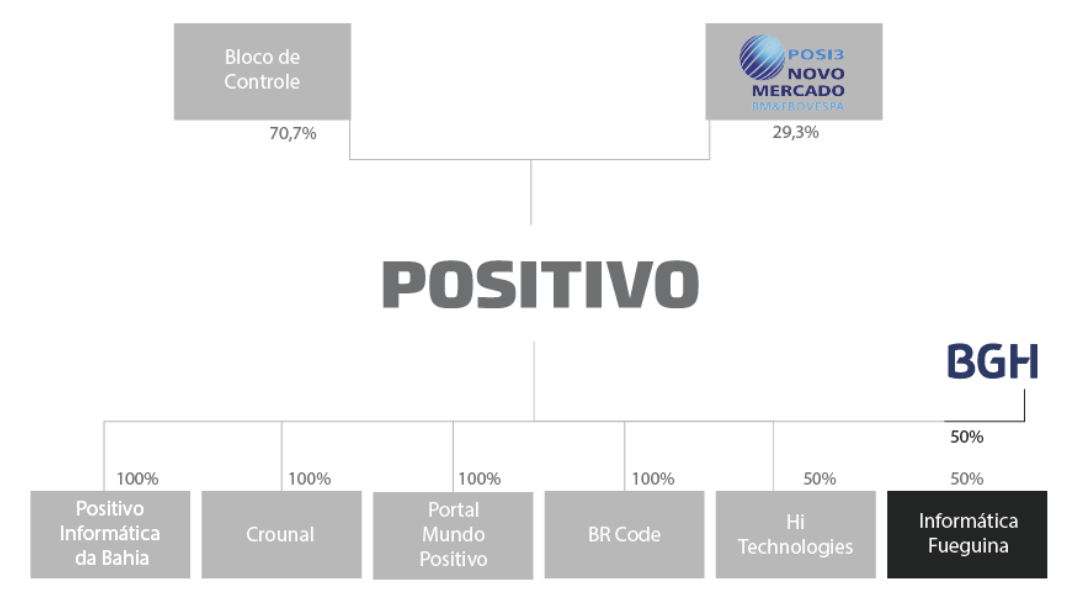
\includegraphics[width=1.0\textwidth]{Img/Corporativo}
\caption{Figura que demonstra o domínio e capital social da \nomeCompletoPositivo{}.}
\par\end{centering}
\end{figure}

Em 2016, a Positivo Tecnologia foi uma das maiores fabricantes de computadores no Brasil, respondendo por 15,3\% do número total de computadores vendidos no mercado brasileiro, de acordo com a IDC. No mesmo período, obtiveram uma participação de 19,9\% do mercado de varejo. Uma parcela substancial da produção de computadores é vendida através de grandes redes de varejo, com as quais o grupo mantém sólido relacionamento comercial, em função principalmente dos preços competitivos, do reconhecimento da marca e assistência técnica.

Adicionalmente, a companhia atua no mercado argentino por meio da marca \nomePositivoAr{}, fruto de uma joint venture com um parceiro local. Em 2015, os computadores \nomePositivoAr{} atingiram uma participação de 9,5\%, segundo a IDC.

No Brasil, a Positivo Tecnologia oferece uma linha completa de dispositivos, incluindo computadores de mesa (desktops e all-in-ones), computadores portáteis (notebooks e netbooks) e tablets, que são produzidos em Manaus (AM). Em 2012, a Companhia ingressou no mercado de telefones celulares, com a oferta de smartphones e messaging phones.

\begin{figure}[h]
\begin{centering}
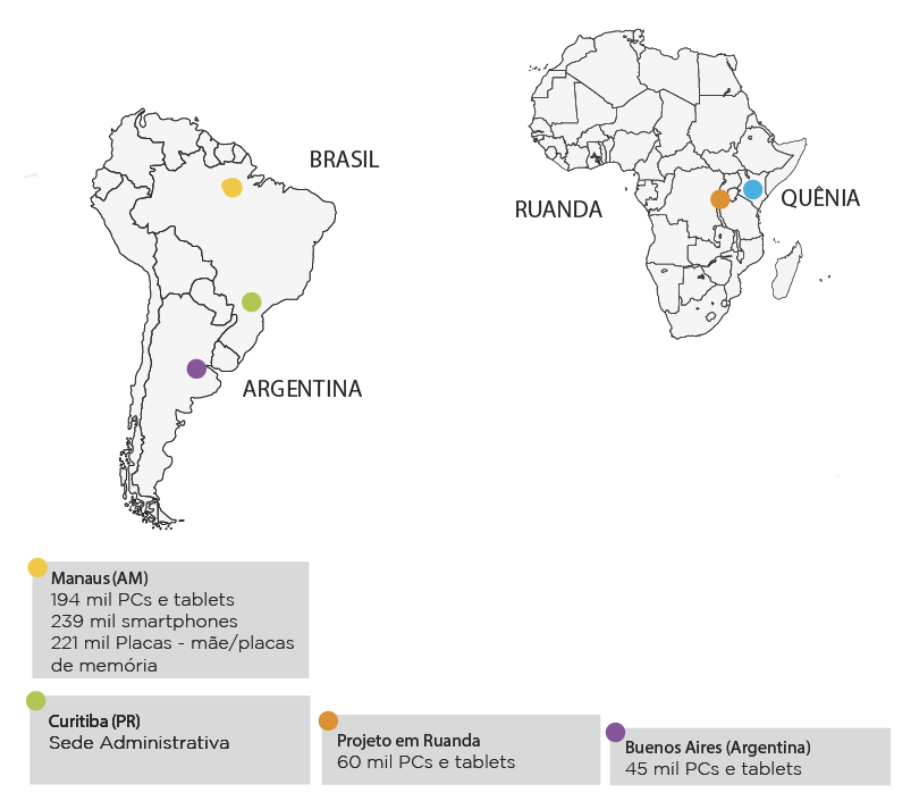
\includegraphics[width=1.0\textwidth]{Img/PositivoMundo}
\caption{Operações da \nomePositivo{} a nível mundial, bastante expressiva na América Latina e observa-se também sítios na África.}
\par\end{centering}
\end{figure}

Além disso, para atendimento e suporte aos milhões de consumidores finais, empresas e órgãos do governo, conta com uma ampla e capacitada rede de assistências técnicas cobrindo a totalidade do território nacional, e com a CRP - Central de Relacionamento Positivo, que registrou em média, 2,9 mil contatos diários em 2016. Grande parte destes contatos se refere a questões básicas sobre uso do computador, sistema operacional ou problemas com conexões, uma vez que muitos dos clientes estão adquirindo seu computador pela primeira vez.

Parcela menor da receita da Companhia provém do Segmento de Tecnologia Educacional, no qual acredita ser líder absoluto no País. A Companhia oferece soluções de infraestrutura e gestão, aplicativos e plataformas educacionais, portais de educação, além de formação de professores e acompanhamento pedagógico. Os portais têm mais de 1,2 milhões de usuários ativos, com modelo de receita recorrente mensal. 

As soluções educacionais da Positivo Tecnologia estão presentes em mais de 14 mil escolas e são exportadas para mais de 40 países. Dentre os principais produtos estão mesas educacionais, dispositivos móveis, lousas interativas, dispositivos de armazenamento e recarga, projetores, acess point, e sistema de gerenciamento de aulas. A Companhia é também distribuidor exclusivo no Brasil de empresas líderes no desenvolvimento e distribuição de software educacional, bem como distribui produtos da LEGO\texttrademark Education no território nacional.

Em 2016, a Companhia ingressou no mercado de tecnologia médica por meio da aquisição de 50\% do capital social da Hi Technologies S.A., empresa com forte foco em P\&D para a oferta de produtos inovadores em saúde.


% ----------------------------------------------------------
% Análise dos clusters
% ----------------------------------------------------------

\chapter{Análise de Variáveis}
Neste capítulo, será feito uma análise passo a passo de cada uma das
variáveis do espaço amostral da base \nomeDaBase{}. Conforme demonstrado
no capítulo \ref{chap:Introducao}.


\section{Status}

\begin{figure}
\begin{centering}
\includegraphics[width=0.8\textwidth]{status_freq}
\par\end{centering}

\caption{\label{fig:FreqStatus}Gráfico de barras de frequência da variável
STATUS.}
\end{figure}
A variável \emph{Status }é aquela de maior interesse na pesquisa de
dados e é a que deve-se prever. Ela identifica quem são os adimplentes
e inadimplentes na base \nomeDaBase{}.

Nota-se, na tabela \ref{tab:StatusNatureza} que 69,3\% da amostra
é Adimplente enquanto 30,7\% é inadimplente, graficamente representado
no gráfico \ref{fig:FreqStatus}. O resultado também pode ser confirmado
pelo comando R:

\begin{minted}{R}
> CrossTable(calvo$STATUS)
\end{minted}

\begin{table}[h]
\centering
\input{Table/status.tex}
\caption{\label{tab:StatusEstado}Análise de frequência relativa da variável \emph{status} na amostra}
\end{table}

\section{Estado (UF)}

Nota-se que cerca 96\% da amostra é de SP, seguido por cerca de 4\%
de MG, o restante dos estados somados representam cerca de 1\%.

\begin{minted}{R}
> CrossTable(calvo$UF, calvo$STATUS, prop.chisq = F, prop.t = F, digits = 2)
\end{minted}

\begin{table}[h]
\centering
\input{Table/status_estado.tex}
\caption{\label{tab:StatusEstado}Tabela de relação entre as variáveis \emph{Status} e \emph{Estado (UF)}}
\end{table}

\section{Escolaridade}

\begin{table}[h]
\centering
\input{Table/status_escolaridade.tex}
\caption{\label{tab:StatusEscolaridade}Tabela de relação entre as variáveis \emph{Status
} e \emph{Escolaridade}}
\end{table}

Nota-se que a maior proporção se encontra nos que possuem escolaridade
Secundária com cerca de 35\% e a menor proporção é de nível de escolaridade
Pós Graduação com 8\%.

Os registros com Pos Graduação possuem o menor índice de Inadimplentes
com 18\%, enquanto os com nível Primário tem 37\% de Inadimplentes.

\section{Estado Civil}

\begin{table}[h]
\centering
\input{Table/status_estciv.tex}
\caption{\label{tab:StatusEstadoCivil}Tabela de relação entre as variáveis \emph{Status
}e \emph{Estado Civil}}
\end{table}

Na tabela \ref{tab:StatusEstadoCivil}, temos Os percentuais individuais dos possíveis valores para a variável estado civil: \emph{solteiro, casado, divorciado, viúvo e outros}. As colunas representam a divisão em \emph{adimplentes} e \emph{inadimplentes}.

Observa-se que a maioria dos tomadores de empréstimos são solteiros com 59\%, enquanto a minoria são outros, com 1\%.

Os maiores inadimplentes são os divorciados com 77\% e os menores inadimplentes são os casados com 15\%.

\section{Renda}

A menor renda que temos é 1 e a maior é 1.380.200,00, através do boxplot
pode-se ver que não temos dados homogêneos, ou seja, temos muitos
outliers:

TODO - imagem do boxplot

Para melhor analisar a renda, a mesma foi discretizada em faixas utilizando
um algoritmo de quebra supervisionado do R:

\begin{lstlisting}
  ksalario             admpl      inad
    [   1,    839) 0.7578000 0.2422000
    [ 839,   1373) 0.7448000 0.2552000
    [1373,   2261) 0.6923846 0.3076154
    [2261,   4021) 0.6810580 0.3189420
    [4021,1380200] 0.5884655 0.4115345
\end{lstlisting}


Com essa divisão em faixas, é possível notar que quanto maior a faixa
de renda, maior a inadimplência.


\section{Natureza}

\begin{table}[h]
\centering
\input{Table/status_natureza.tex}
\caption{\label{tab:StatusNatureza}Tabela de relação entre as variáveis \emph{Status
}e \emph{Natureza}}
\end{table}

É evidenciado na tabela \ref{tab:StatusNatureza} os percentuais individuais dada a natureza do vínculo empregatício
do indivíduo com relação ao fato de ele encontrar-se em adimplência ou inadimplência. Nota-se que para determinadas categorias 
há maior presença de um ou outro \emph{status}. 

Na figura \ref{fig:FreqStatusVsNatureza}, demonstra-se todas as diferentes classes da variável categorica \emph{natureza} em relação ao status percentual na amostra. Evidencia-se uma grande predominância de poucas classes no espaço amostral.

\begin{center}
\begin{figure}
\begin{centering}
\includegraphics[width=0.85\textwidth]{natureza_vs_status}
\par\end{centering}

\caption{\label{fig:FreqStatusVsNatureza}Gráfico de barras de frequência da
  variável \emph{status} para a categoria \emph{natureza}.}
\end{figure}

\par\end{center}

Os tomadores de empréstimos de Natureza de Renda \emph{empregado} são os
mais inadimplentes com 40\% e os menos inadimplentes são os \emph{profissionais
liberais} com 1\%. O resultado também pode ser confirmado pelo comando
R:

\begin{minted}{R}
> CrossTable(calvo$STATUS)
\end{minted}


\chapter{Árvore de Decisão}
A árvore de decisão, é um mecanismo que permite entendermos uma variável,
estimando seu valor baseado numa regressão, na qual o espaço é subdividido
em duas partes a cada nível. Presta-se assim, a uma caracterização
binária da amostra de dados de entrada.


\section{Árvore gerada}

Utilizando o seed 5668 os dados foram separados em duas amostras aleatórias
de 12500 observações cada.

Através do método CART foi gerada a seguinte árvore com a amostra
de aprendizado:

\begin{center}
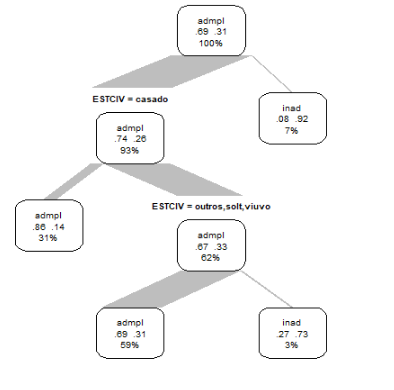
\includegraphics[width=0.9\textwidth]{CartTree}
\par\end{center}

É possível notar que as variáveis mais significantes para a classificação
foram Natureza e Estado Civil. 

\begin{minted}{R}
> printcp(ac1)
\end{minted}

\begin{lstlisting}
Classification tree:
rpart(formula = STATUS ~ UF + ESCOLARIDADE + ESTCIV + FAIXARENDA + 
    NATUREZA, data = calvo.lrn)
 
Variables actually used in tree construction:
[1] ESTCIV   NATUREZA
 
Root node error: 3861/12500 = 0.30888
 
n= 12500 
 
        CP nsplit rel error  xerror     xstd
1 0.182595      0   1.00000 1.00000 0.013379
2 0.018778      1   0.81740 0.81740 0.012580
3 0.010000      3   0.77985 0.77985 0.012383
\end{lstlisting}


Através dos valores CP é possível verificar que os erros para a amostra
de aprendizado foram de 31\% e a menor taxa de erro se encontra no
nó 3 com 78\%, portando não é necessário podar a árvore. 


\section{Validação com Amostra Teste}

\begin{minted}{R}
> CrossTable(calvo.tst$STATUS, yhat_tst, prop.chisq = F, prop.t = F, digits = 2)
\end{minted}

\begin{lstlisting}
   Cell Contents
|-------------------------|
|                       N |
|           N / Row Total |
|           N / Col Total |
|-------------------------|
 
 
Total Observations in Table:  12500 
 
 
                 | yhat_tst 
calvo.tst$STATUS |     admpl |      inad | Row Total | 
-----------------|-----------|-----------|-----------|
           admpl |      8534 |       163 |      8697 | 
                 |      0.98 |      0.02 |      0.70 | 
                 |      0.75 |      0.15 |           | 
-----------------|-----------|-----------|-----------|
            inad |      2869 |       934 |      3803 | 
                 |      0.75 |      0.25 |      0.30 | 
                 |      0.25 |      0.85 |           | 
-----------------|-----------|-----------|-----------|
    Column Total |     11403 |      1097 |     12500 | 
                 |      0.91 |      0.09 |           | 
-----------------|-----------|-----------|-----------|
\end{lstlisting}


Pode-se notar que existe 20\% de erro na amostra de teste, sendo maior
na classificação de adimplentes para inadimplentes (25\%). 


% ----------------------------------------------------------
% Finaliza a parte no bookmark do PDF
% para que se inicie o bookmark na raiz
% e adiciona espaço de parte no Sumário
% ----------------------------------------------------------
\phantompart

% ---
% Conclusão - Recomendação de qual protótipo
% ---
\chapter{Conclusões}
% ---

%Placeholder
%\label{chap:conclusao}

\begin{figure}
\begin{centering}
\subfloat[\label{fig:prototipo-familia}Conforto,
espaço e filhos.]{\begin{centering}
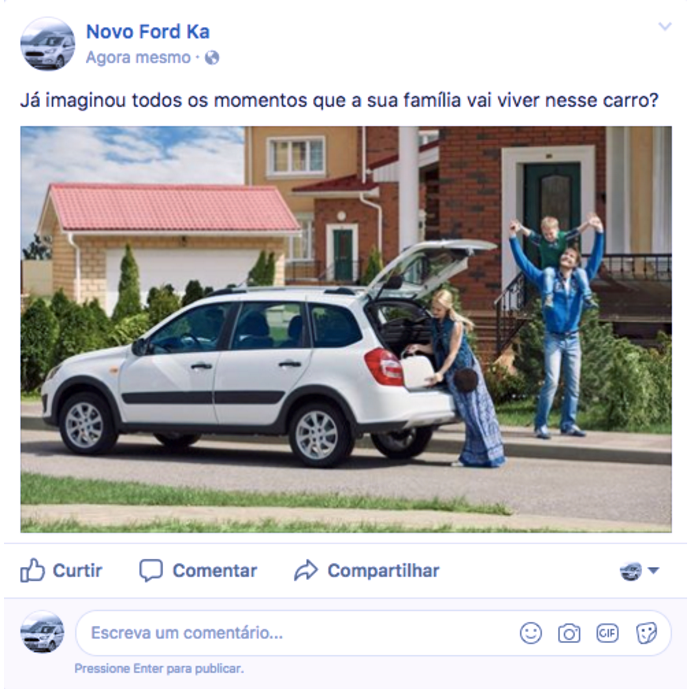
\includegraphics[height=0.30\textheight]{Imagens/p1_familia}~~
\par\end{centering}
}\subfloat[\label{fig:prototipo-versatil}Aborda o efeito versátil do carro.]{\begin{centering}
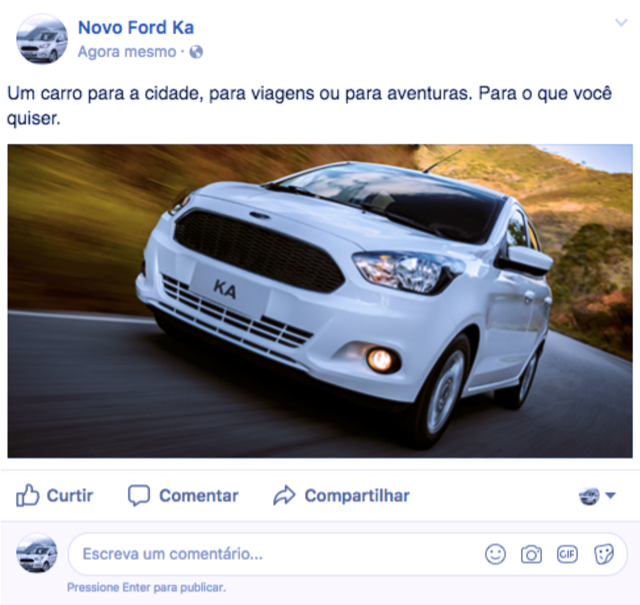
\includegraphics[height=0.30\textheight]{Imagens/p1_prototipo}
\par\end{centering}
}
\par\end{centering}
\caption{Peças ilustrativas de uma campanha em formato carrossel.}
\end{figure}

De acordo com o desenvolvido no capítulo \ref{chap:analise}, com
as tabelas \ref{tab:prototipo-vs-cluster} e \ref{tab:prototipo-analise},
contrasta a homogeneidade dos protótipo 2 e 3 à heterogeneidade do
protótipo 1. À primeira vista, percebe-se que os três protótipos possuem
proporções da população muito parecidas, entretanto há uma grande
diferença entre o protótipo 1, heterogêneo, com os demais protótipos.
Isto é, a possibilidade de uma campanha publicitária informativa unida
a transformativas que possibilitarão, se escolhido o protótipo 1,
abranger também os clusters \nomeCc{} e \nomeCb{}, dado que pela
própria heterogeneidade do protótipo 1, certas propagandas que apelam
para determinadas características do protótipo podem aumentar a aceitação
de uma campanha baseada neste protótipo.

\begin{table}
\begin{centering}
\begin{tabular}{c|>{\centering}p{0.28\textwidth}|>{\centering}p{0.28\textwidth}|>{\centering}p{0.28\textwidth}}
\hline 
 & Protótipo 1 & Protótipo 2 & Protótipo 3\tabularnewline
\hline 
Bom & Preferido entre \nomeCa{} e \nomeCd{}. & Amplamente preferido pelo cluster dos \nomeCc{}. & Amplamente preferido pelos \nomeCb{}, focados em Imagem.\tabularnewline
\hline 
Ruim & Somente uma estratégia de marketing não é suficiente, dada a sua heterogeneidade
e várias afinidades. & Difícil para a publicidade porque se mostra indiferente a carros.
Importam-se apenas com o preço. & Uma campanha publicitária em Imagem somente não gera interesse de
outros clusters.\tabularnewline
\hline 
\end{tabular}
\par\end{centering}
\caption{\label{tab:prototipo-analise}Vantagens e desvantagens por protótipos.}
\end{table}


Por exemplo, se uma campanha publicitária apelar de maneira informativa
e transformativa para os aspectos de Imagem e Utilitário do carro,
é possível abranger os clusters mencionados anteriormente, sustentando
assim uma aceitação maior por parte da população. Ou seja, escolhe-se
a versatilidade do protótipo 1, numa eventual campanha publicitária
como elemento.

\begin{figure}
\begin{centering}
\subfloat[\label{fig:painel-cambio}Acabamento e câmbio.]{\begin{centering}
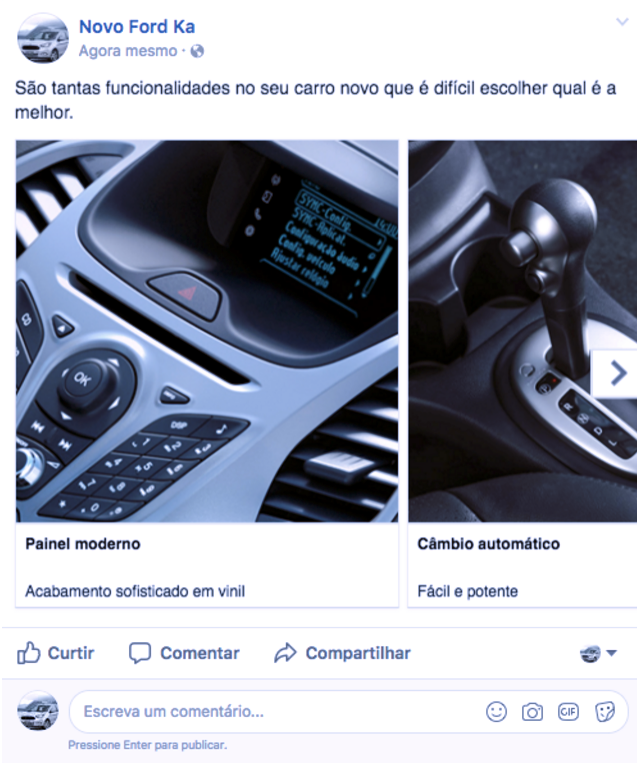
\includegraphics[height=0.34\textheight]{Imagens/p1_interior}
\par\end{centering}
}~~\subfloat[\label{fig:ar}Ar-condicionado.]{\begin{centering}
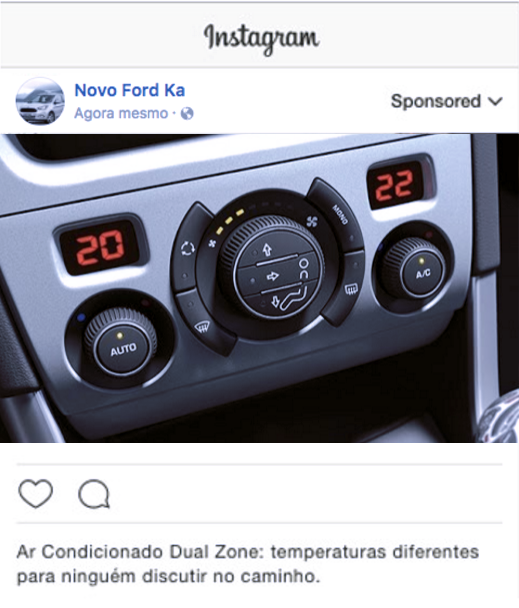
\includegraphics[height=0.34\textheight]{Imagens/p1_interior_painel}
\par\end{centering}
}
\par\end{centering}
\caption{Peças multifuncionais para Utilitário e Imagem.}
\end{figure}


\section{Recomendações para Campanha Publicitária}

Com base nas características analisadas dos grupos \nomeCa{} e \nomeCd{}
será feita uma combinação de campanhas publicitárias: para os \nomeCa{},
uma campanha transformativa mesclando os três atributos: Imagem, Utilitário
e Preço. Para os \nomeCd{}, uma campanha ressaltando o carro como
utilitário. Por se tratar de dois grupos diferentes vamos destacar
multifuncionalidade, tecnologia, versatilidade e conforto.

É possível uma campanh que foque nas seguintes características: confortável
e espaçoso. O público-alvo seriam os \nomeCd{} que preferem carros
como bens utilitários, destacando o porta-malas espaçoso para a família.
Os \nomeCd{} são formados predominantemente por mulheres com filhos,
por isso o destaque a família, na figura \ref{fig:prototipo-familia}.

A campanha com formato em carrossel irá abordar a característica de
multifuncionalidade. A publicidade tem foco nos \nomeCa{} combinando
funcionalidades (Utilitário) que valorizem o carro (Preço) e que tragam
mais sofisticação (Imagem), como vê-se nas figuras \ref{fig:painel-cambio}
e \ref{fig:ar}.

Finalmente, a figura \ref{fig:prototipo-versatil} seria veiculada
em formato vídeo, tanto em Facebook quanto na televisão. Destaca a
versatilidade do Ford Ka\texttrademark, valorizando o fato de ser
um carro potente (Utilitário) e ainda assim econômico (Preço). Em
televisão, dá-se preferência é por intervalos de jogos de futebol
buscando atingir um público predominantemente masculino que gosta
de esportes e aventuras. 



% ----------------------------------------------------------
% ELEMENTOS PÓS-TEXTUAIS
% ----------------------------------------------------------
\postextual
% ----------------------------------------------------------

% ----------------------------------------------------------
% Referências bibliográficas
% ----------------------------------------------------------
\bibliography{referencias}

% ----------------------------------------------------------
% Glossário
% ----------------------------------------------------------
%
% Consulte o manual da classe abntex2 para orientações sobre o glossário.
%
%\glossary

% ----------------------------------------------------------
% Apêndices
% ----------------------------------------------------------

% ---
% Inicia os apêndices
% ---
%\begin{apendicesenv}

%% Imprime uma página indicando o início dos apêndices
%\partapendices

%% ----------------------------------------------------------
%\chapter{Quisque libero justo}
%% ----------------------------------------------------------

%\lipsum[50]

%% ----------------------------------------------------------
%\chapter{Nullam elementum urna vel imperdiet sodales elit ipsum pharetra ligula
%ac pretium ante justo a nulla curabitur tristique arcu eu metus}
%% ----------------------------------------------------------
%\lipsum[55-57]

%\end{apendicesenv}
% ---


% ----------------------------------------------------------
% Anexos
% ----------------------------------------------------------

% ---
% Inicia os anexos
% ---
%\begin{anexosenv}

%% Imprime uma página indicando o início dos anexos
%\partanexos

%% ---
%\chapter{Morbi ultrices rutrum lorem.}
%% ---
%\lipsum[30]

%% ---
%\chapter{Cras non urna sed feugiat cum sociis natoque penatibus et magnis dis
%parturient montes nascetur ridiculus mus}
%% ---

%\lipsum[31]

%% ---
%\chapter{Fusce facilisis lacinia dui}
%% ---

%\lipsum[32]

%\end{anexosenv}

%---------------------------------------------------------------------
% INDICE REMISSIVO
%---------------------------------------------------------------------
\phantompart
\printindex
%---------------------------------------------------------------------

\end{document}
